\documentclass[11pt,xcolor=svgnames]{beamer}
\usepackage{dsfont,natbib,setspace,changepage,multirow}
\mode<presentation>

% replaces beamer foot with simple page number
\setbeamertemplate{navigation symbols}{}
\setbeamerfont{frametitle}{series=\bfseries,size=\normalsize}
\setbeamercolor{frametitle}{fg=Black}

\setbeamertemplate{footline}{
   \raisebox{5pt}{\makebox[\paperwidth]{\hfill\makebox[20pt]{\color{gray}\scriptsize\insertframenumber}}}}

\usepackage{algorithm}
\usepackage{algorithmic}

% colors
\newcommand{\theme}{\color{DarkBlue}}
\newcommand{\bk}{\color{black}}
\newcommand{\rd}{\color{red}}
\newcommand{\fg}{\color{ForestGreen}}
\newcommand{\bl}{\color{blue}}
\newcommand{\gr}{\color{black!50}}
\newcommand{\sg}{\color{DarkSlateGray}}
\newcommand{\nv}{\color{Navy}}
\setbeamercolor{itemize item}{fg=gray}

% common math markups
\newcommand{\bs}[1]{\boldsymbol{#1}}
\newcommand{\mc}[1]{\mathcal{#1}}
\newcommand{\mr}[1]{\mathrm{#1}}
\newcommand{\bm}[1]{\mathbf{#1}}
\newcommand{\ds}[1]{\mathds{#1}}
\newcommand{\indep}{\perp\!\!\!\perp}
\def\plus{\texttt{+}}
\def\minus{\texttt{-}}

% spacing and style shorthand
\setstretch{1.1}

\begin{document}

\setcounter{page}{0}
{ 
\begin{frame}[plain]
\begin{center}

{\bf \LARGE \theme Regularized Estimation of \\\vskip .25cm Hockey Player Performance}
\end{center}

\vskip 1cm
~~~~~~~~{\bf Bobby Gramacy}, Chicago Booth
\vskip .1cm
~~~~~~~~{\bf Matt Taddy},  Microsoft Research and Chicago Booth~~~~
%{\gr \texttt{faculty.chicagobooth.edu/matt.taddy/research}}

\vskip .1cm
{\color{black!70} ~~~~~~~~~~~with  Sen Tian (NYU) and Shane Jenson (Wharton)}


\end{frame} }

\begin{frame}
{Plus-Minus}

PM is a running count of, for every goal, a +1 for those on \\the scoring team and -1 for those on the team scored upon.

\vskip .25cm
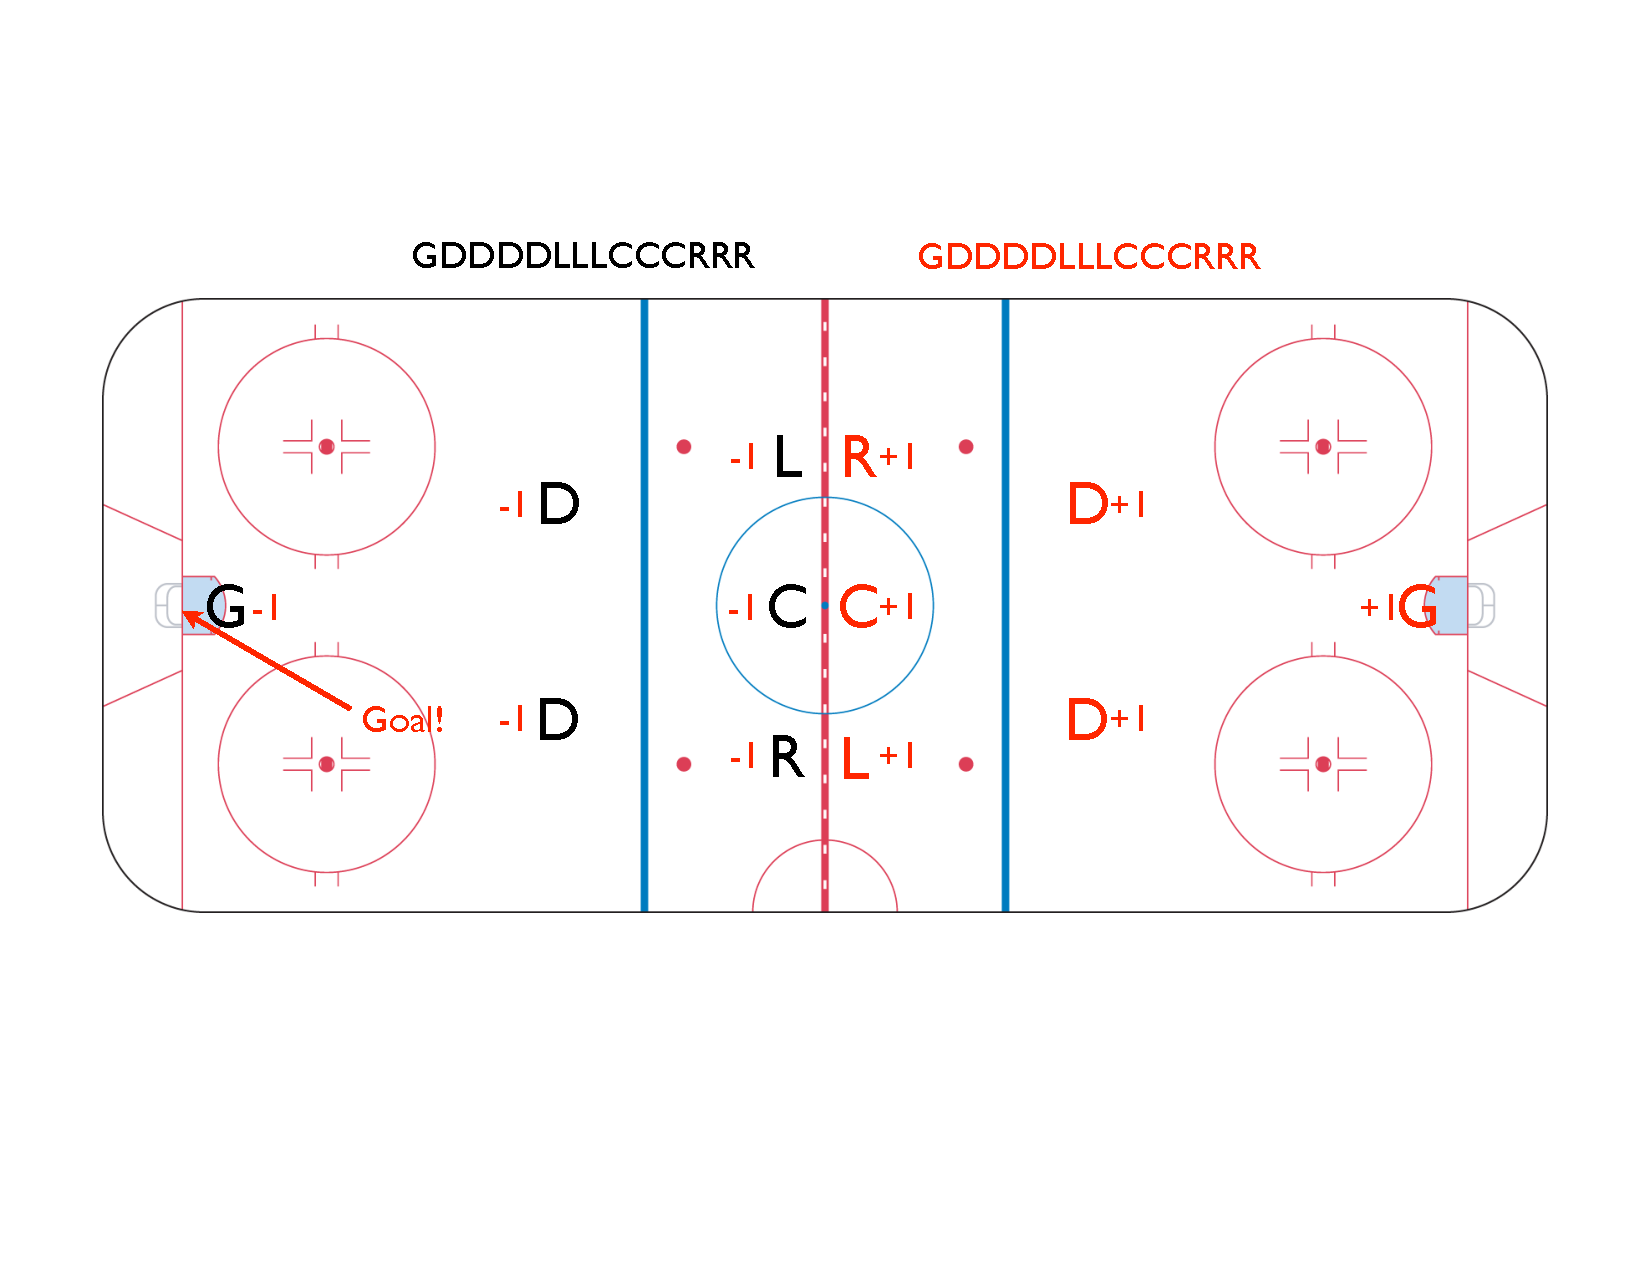
\includegraphics[width=\textwidth]{figures/rink_goal.pdf}

It doesn't quite measure player quality, as we haven't controlled for the effects of teammate and opponent quality (or anything else).

\end{frame}

\begin{frame}
{A Regression version of PM}

Set up a `response' variable:\\
~~~~ $y_i = +1$ for a \textit{home} team goal, \\
~~~~~$y_i = -1$ for an \textit{away} team goal.

\vskip .25cm
We're interested in how individual players affect
\[
{\theme q_i =
\mathrm{p}(y_i = 1) =  \mathrm{p}(\text{home~team~scored~goal}~i)}
\]

The standard model for such problems is logistic regression, say
\[
\log\left[\frac{q_{i}}{1-q_{i}}\right] = \alpha + \beta_{HG} + \beta_{HD} ... +\beta_{HR} - \beta_{AG} - ... - \beta_{AR}
\]
where $\beta_{HG}$ is Home-Goalie and $\beta_{AR}$ is Away-Right-wing, etc. 

\vskip .25cm\gr
Then, for player $j$ and given a goal was scored, $e^{\beta_j}$ is the multiplier\\ on odds that it was scored by his team if he's on the ice. 
\end{frame}

\begin{frame}

We actually use a larger regression model:
\[\theme 
\log\left[\frac{q_{i}}{1-q_{i}}\right] = \alpha + \mathbf{u}_i'\boldsymbol{\gamma} +
\mathbf{v}_i'\boldsymbol{\varphi} + \mathbf{x}_i'\boldsymbol{\beta}_0 {\gr +
(\mathbf{x}_i\circ\mathbf{s}_i)'(\boldsymbol{\beta}_s + p_i \boldsymbol{\beta}_{p})}
\]
where
\begin{itemize}
\item $\mathbf{u}_i$ holds indicators for each team-season,
\item $\mathbf{v}_i$ holds indicators for various special-teams scenarios,
\item 
$\mathbf{x}_i$ contains player-presence indicator,
\end{itemize}
All of these indicators are +1 for home and -1 for away.

\vskip .25cm
Then $\beta_j$ measures player effect after {\theme controlling} for team strength (e.g., coach or schedule) and on-ice scenarios (e.g., PP or PK).


\vskip .25cm {\gr We also allow deviations in the player effects for specific seasons ($s_{it}$) and in the playoffs ($p_{it}$), but these are seldom `significant'.}

\vskip -.5cm
\end{frame}

\begin{frame}
{Regularization}

Instead of minimizing deviance, we minimize deviance {\it plus penalty $\lambda|\beta_j|$ on the size of each $\beta_j$ coefficient}.  {\gr This is called the LASSO.}

\vskip -.15cm
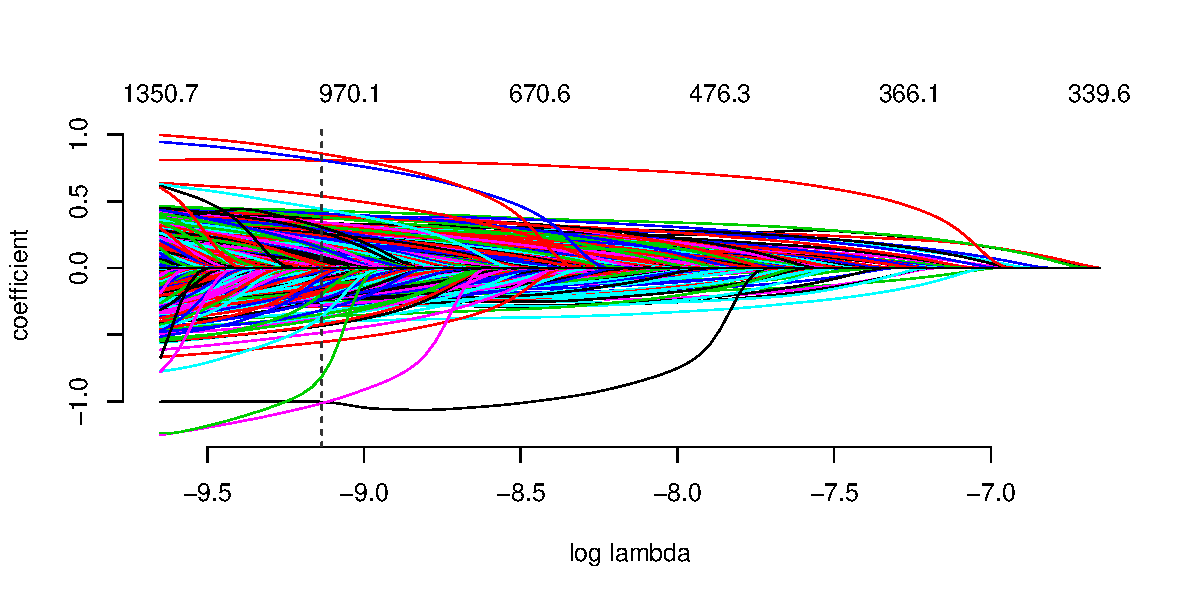
\includegraphics[width=\textwidth]{figures/pathplot.pdf}

\vskip -.1cm
Enumerate a `path' of models for different $\lambda$, and use the one that predicts best out-of-sample. {\theme This is how modern statistics works.}

{\gr See the {\tt gamlr} package for R, and {\tt help(hockey)} for this example.  }

\vskip -.5cm

\end{frame}

\begin{frame}
{Partial PM and FP}

We use the estimated logistic regression model to produce `partial' 
(i.e., without effect of confounders) versions of standard statistics.
\vskip .1cm
\begin{itemize}
\item For-Probability: $\theme \displaystyle PFP_j = \frac{e^{\beta_j}}{(1+e^{\beta_j})}$
\item[]
\item Plus-Minus: $ \theme PPM_j = G_j PFP_j - G_j(1-PFP_j)$\\{ ~~~where $G_j$ is the total goals with player $j$ on-ice.}
\end{itemize}

\vskip .2cm
PFP measures the player's average contribution, and PPM scales this up by \# of goals (which is a rough surrogate for time-on-ice).

\vskip .2cm
{\gr We also fit models for non-goal response $y_i$, like shots or corsi events.  This gives partial versions of stats based on those metrics.}

\end{frame}

\begin{frame}

\scriptsize
	\begin{tabular}{r c c c|r r r r }
		\multicolumn{8}{l}{\bf Goal-based performance analysis, ordered by PPM: Studs} \\ \\
		Rank & Player & Season  & Team & PFP & FP & PPM & PM \\ \hline
		\rule{0pt}{4ex} 
		1&PETER FORSBERG&2002-2003&COL&0.68&0.77&55.52&85\\
		2&SIDNEY CROSBY&2009-2010&PIT&0.60&0.64&43.47&60\\
		3&DOMINIK HASEK&2005-2006&OTT&0.59&0.67&42.45&80\\
		4&SIDNEY CROSBY&2008-2009&PIT&0.60&0.61&42.26&48\\
		5&SIDNEY CROSBY&2005-2006&PIT&0.60&0.62&41.86&52\\
		6&PETER FORSBERG&2005-2006&PHI&0.68&0.77&40.67&61\\
		7&PAVEL DATSYUK&2007-2008&DET&0.60&0.72&39.49&87\\
		8&PAVEL DATSYUK&2008-2009&DET&0.60&0.67&39.49&69\\
		9&SIDNEY CROSBY&2006-2007&PIT&0.60&0.72&35.62&79\\
		10&MARK STREIT&2008-2009&NYI&0.59&0.56&35.08&24\\
		11&MATT MOULSON&2011-2012&NYI&0.60&0.61&34.92&37\\
		12&LUBOMIR VISNOVSKY&2010-2011&ANA&0.58&0.66&34.52&70\\
		13&ALEX OVECHKIN&2008-2009&WAS&0.57&0.66&34.46&80\\
		14&JOE THORNTON&2009-2010&SJS&0.60&0.65&33.91&52\\
		15&JOE THORNTON&2010-2011&SJS&0.60&0.64&33.91&48\\
		16&ONDREJ PALAT&2013-2014&TAM&0.64&0.66&32.75&37\\
		17&PAVEL DATSYUK&2006-2007&DET&0.60&0.71&32.61&70\\
		18&JOE THORNTON&2002-2003&BOS&0.60&0.64&32.17&47\\
		19&JOE THORNTON&2007-2008&SJS&0.60&0.71&32.17&69\\
		20&ANDREI MARKOV&2007-2008&MON&0.57&0.60&31.9&47\\
\end{tabular}
\end{frame}

\begin{frame}
\scriptsize
	\begin{tabular}{r c c c|r r r r }
		\multicolumn{8}{l}{\bf\theme Goal-based performance analysis, ordered by PPM: Duds} \\ \\
		Rank & Player & Season  & Team & PFP & FP & PPM & PM \\ \hline
		\rule{0pt}{4ex} 

		10184&PATRICK LALIME&2008-2009&BUF&0.43&0.44&-15.79&-15\\
		10185&JACK JOHNSON&2007-2008&LOS&0.45&0.39&-15.82&-34\\
		10186&BRETT CLARK&2011-2012&TAM&0.44&0.35&-16.93&-47\\
		10187&NICLAS HAVELID&2008-2009&ATL&0.45&0.39&-16.97&-40\\
		10188&JACK JOHNSON&2010-2011&LOS&0.45&0.53&-17.21&9\\
		10189&JACK JOHNSON&2011-2012&LOS&0.45&0.5&-17.21&-1\\
		10190&P. J. AXELSSON&2008-2009&BOS&0.41&0.49&-17.35&-1\\
		10191&BRYAN ALLEN&2006-2007&FLA&0.45&0.45&-17.9&-17\\
		10192&JACK JOHNSON&2009-2010&LOS&0.45&0.49&-19.46&-4\\
		10193&PATRICK LALIME&2005-2006&STL&0.43&0.40&-19.77&-29\\
		10194&ALEXANDER EDLER&2013-2014&VAN&0.37&0.27&-20.49&-35\\
		10195&PATRICK LALIME&2007-2008&CHI&0.43&0.49&-22.29&-4\\
		10196&TIM THOMAS&2009-2010&BOS&0.43&0.46&-24.22&-16\\
		10197&ANDREJ MESZAROS&2006-2007&OTT&0.42&0.48&-27.32&-6\\
		10198&BRYCE SALVADOR&2008-2009&NJD&0.35&0.37&-34.4&-31\\
		10199&PATRICK LALIME&2002-2003&OTT&0.43&0.58&-37.81&47\\
		10200&PATRICK LALIME&2003-2004&OTT&0.43&0.56&-37.81&37\\
		10201&NICLAS HAVELID&2006-2007&ATL&0.34&0.44&-62.64&-22\\
		10202&NICLAS HAVELID&2005-2006&ATL&0.33&0.40&-65.94&-41\\
		10203&JAY BOUWMEESTER&2005-2006&FLA&0.33&0.42&-69.62&-32\\
	\end{tabular}

\end{frame}

\begin{frame}

For abundant detail and analysis, see our handbook chapter\\ {\theme Hockey Performance via Regression} {\gr by Gramacy, Taddy, and Tian.}

\vskip .5cm  
e.g., look at average player salary by standard and partial statistics

\begin{figure}[tbh]
    \centering
    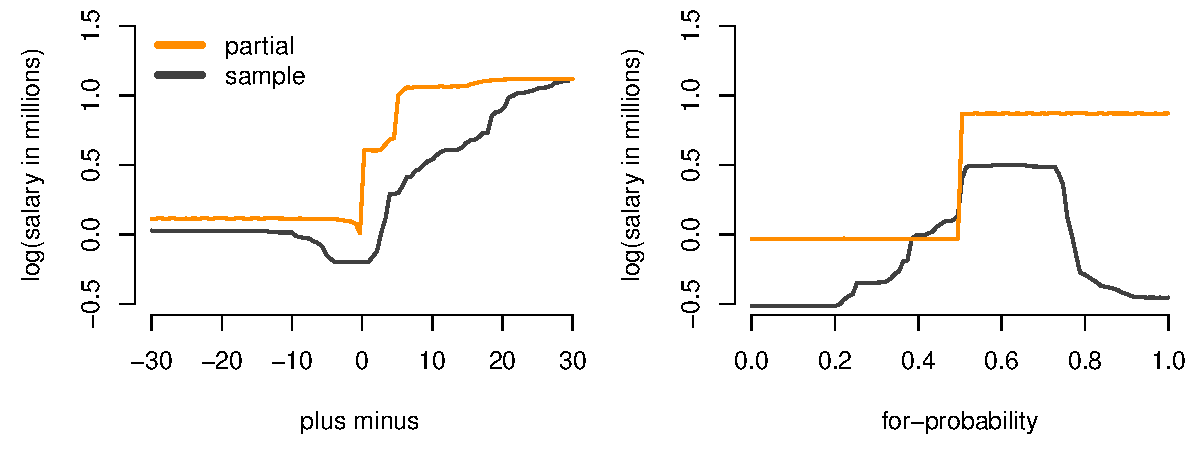
\includegraphics[width=\textwidth]{../crcpaper/figures/salreg-goals.pdf}
 \end{figure}

\end{frame}

\begin{frame}{Bargains!}

Top-15 undervalued players in 2013-2014
\begin{table}
	\centering\footnotesize
	\begin{tabular}{r c c r   }
		Rank & Player & Team & Goals per million  \\ 
		\hline\rule{0pt}{4ex} 
		1&ONDREJ PALAT&TAM&58.27\\
		2&RYAN NUGENT-HOPKINS&EDM&19.81\\
		3&GABRIEL LANDESKOG&COL&16.74\\
		4&TYLER TOFFOLI&LOS&16.72\\
		5&GUSTAV NYQUIST&DET&9.08\\
		6&JADEN SCHWARTZ&STL&8.43\\
		7&ERIC FEHR&WAS&7.51\\
		8&ANDREW MACDONALD&NYI&7.48\\
		9&BENOIT POULIOT&NYR&6.43\\
		10&BRAD BOYES&FLA&6.01\\
		11&TOMAS TATAR&DET&5.83\\
		12&AL MONTOYA&WPG&5.79\\
		13&BRANDON SAAD&CHI&5.5\\
		14&FRANS NIELSEN&NYI&5.5\\
		15&JAROMIR JAGR&NJD&4.73
	\end{tabular}
\end{table}

\end{frame}

\begin{frame}

We also include comparison of shot and goal-based metrics:
\vskip .2cm
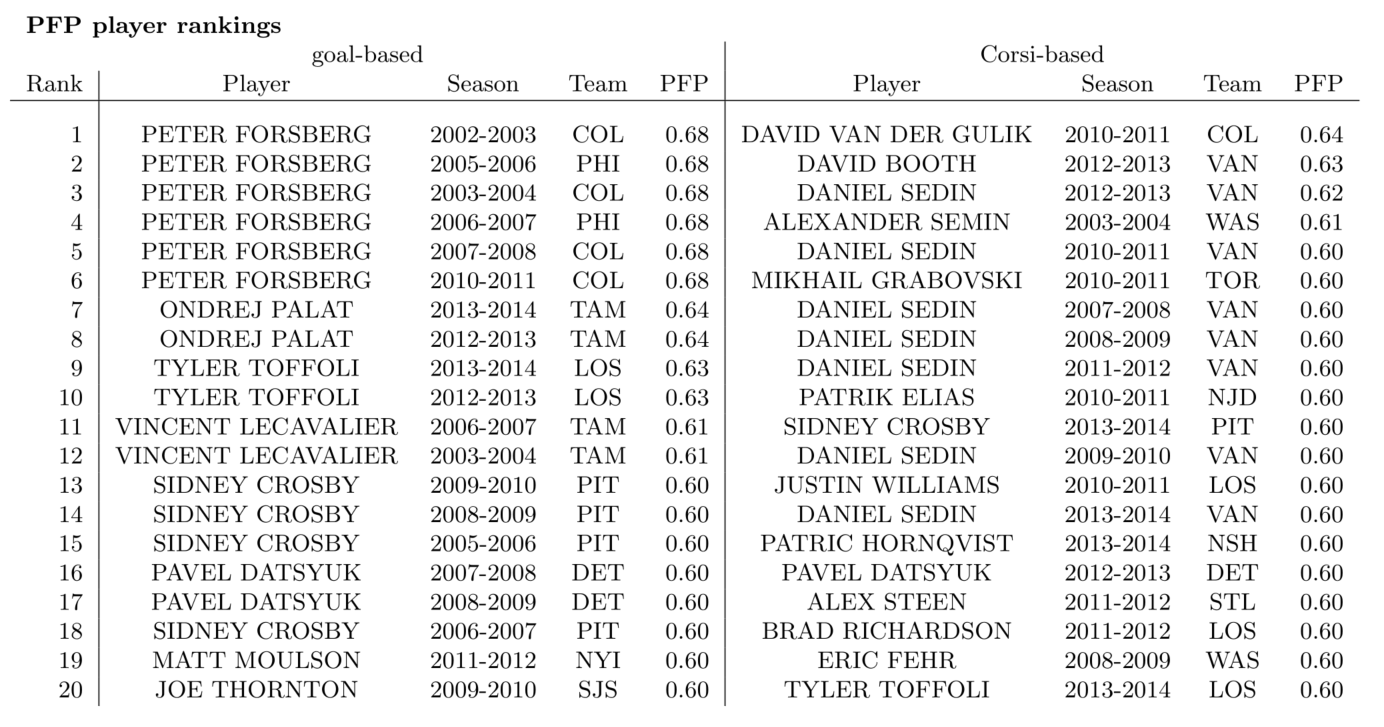
\includegraphics[width=\textwidth]{figures/pfpCapture.PNG}

\vskip .1cm \hfill and much else.
\end{frame}

\begin{frame}[fragile]
{Wrap-up}

The model is very transparent and easy to estimate.  

\vskip .25cm
Check out {\tt gamlr} and the {\tt hockey} example:

\vskip -.25cm
{\small \color{black!75}
\begin{verbatim}
    data(hockey)
    x <- cBind(config,team,player)
    y <- goal$homegoal
    fit <- gamlr(x, y, free=1:(ncol(config)+ncol(team)),
                    standardize=FALSE, family="binomial")
\end{verbatim}		 }

We take no stand about what stats lead to wins, \\
and don't attempt to model full game action. 

\vskip .25cm
 But this simple regression tells you a lot about who is contributing.


\vskip 1cm\hfill
{\LARGE\theme\bf Thanks!}

\end{frame}

\end{document}